\documentclass[10pt,a4paper]{article}
\usepackage[utf8]{inputenc}
\usepackage[spanish]{babel}
\usepackage{amsmath}
\usepackage{amsfonts}
\usepackage{amssymb}
\usepackage[T1]{fontenc} 
\usepackage[left=2.00cm, right=2.00cm, top=2.00cm, bottom=2.00cm]{geometry}
\usepackage{acronym}
\usepackage{listings}
\usepackage{graphicx}
\graphicspath{ {images/} }
\usepackage{hyperref}

\usepackage{multirow}
\usepackage[table,xcdraw]{xcolor}

\usepackage[export]{adjustbox}
\usepackage{subcaption}

%%Sobre el código
\usepackage{xcolor}
\usepackage{xparse}
\NewDocumentCommand{\codeword}{v}{%
	\texttt{\textcolor{blue}{#1}}%
}

\setlength{\parindent}{1em}
\setlength{\parskip}{1em}

\spanishdecimal{.}




\title{
Práctica 3\\
\large Aprendizaje Automático \\
}

\author{
Alejandro Palencia Blanco\\
}

\date{30/05/2021}



\begin{document}

\maketitle

\newpage

\tableofcontents

\newpage

\section{Problema de Regresión}

\subsection{Descripción del problema}

El problema consiste en predecir la temperatura crítica de materiales superconductores. El conjunto de datos del que disponemos contiene 21263 superconductores de los cuales se han extraído 81 características. Estas características, a su vez, podemos clasificarlos en 8 subgrupos de 10 atributos según la propiedad sobre la que nos dan información (excepto la característica \textit{number of elements}, que no pertenece a ningún subgrupo). Estos subgrupos son: \textit{atomic mass}, \textit{fie}, \textit{atomic radius}, \textit{density}, \textit{electron affinity}, \textit{fusion heat}, \textit{thermal conductivity} y \textit{valence}. Dentro de cada subgrupo, las características representan valores de interés como la media, la desviación típica, la entropía o el rango.

Como la variable a predecir, temperatura crítica, es una variable continua, podemos plantear un problema de regresión sobre el conjunto de datos para intentar predecir su valor. En el problema no se especifica la unidad en la que se expresan las temperaturas críticas de los elementos del conjunto de datos. Aun así, como muchos de estos materiales adquieren esta capacidad de conducir corriente eléctrica sin pérdida de energía a temperaturas cercanas al cero absoluto, y muchas de las temperaturas críticas que encontramos en el conjunto de datos son ligeramente superiores a cero, deduzco que están expresadas en grados Kelvin. Por tanto, los valores que pueden tomar son mayores o iguales que 0.

Los elementos que constituyen este problema son los siguientes:

\begin{itemize}
	\item $X$: Conjunto de vectores con 81 valores numéricos que representan las características de un superconductor anteriormente descritos.
	\item $Y$: Conjunto de temperaturas críticas que pueden tener asociadas cada uno de los superconductores.
	\item $f$: Función objetivo que asigna a cada vector de la población $X$ la temperatura crítica del superconductor al que representa.
\end{itemize}

Es importante comentar que nada nos garantiza que nuestra hipótesis final prediga valores de temperaturas críticas no negativos (aunque esto esté en contra de las leyes físicas). Por ello, el conjunto $Y$ de posibles temperaturas críticas no está restringido únicamente al intervalo $[0,+\infty[$, sino que está constituido por toda la recta real.






\subsection{Generación de conjuntos de entrenamiento, validación y test}

Partimos de un único archivo \codeword{train.csv} (que he renombrado a \codeword{regression.csv}) con todos los datos, luego solo hay que generar los conjuntos de entrenamiento y test a partir del mismo. Se puede comprobar que no hay datos faltantes, pues al leer los datos, no he tenido ningún error al almacenarlos como arrays de \codeword{numpy} de tipo \codeword{float64}.

Para generar ambos conjuntos, utilizo la función \codeword{train_test_split} indicando que el 20\% de los datos vayan a parar al conjunto de test y el 80\% restante a entrenamiento. Esta separación se hace de forma aleatoria fijando una semilla concreta para que sea la misma en sucesivas ejecuciones. El conjunto de test lo dejamos intacto hasta llegar al último apartado y a partir de ahora pasamos a trabajar con el conjunto de entrenamiento.

En este apartado no obtenemos ningún conjunto de validación. Posteriormente, cuando se lleve a cabo la estimación de hiperparámetros, dividiremos el conjunto de entrenamiento en 5 \textit{folds} para aplicar validación cruzada.




\subsection{Visualización del conjunto de entrenamiento}

Con el objetivo de entender mejor los datos contenidos en el conjunto de entrenamiento, he elaborado dos histogramas con las temperaturas críticas de los superconductores y he visualizado los datos en un espacio bidimensional aplicando los algoritmos PCA (\textit{Principal Component Analysis}) y t-SNE (\textit{t-distributed Stochastic Neighbor Embedding}).

Para elaborar los histogramas, he particionado el intervalo $[0,185]$ (que contiene todas las temperaturas críticas presentes en el conjunto de entrenamiento) en 37 subintervalos de longitud 5. La diferencia entre ambos histogramas es el tipo de frecuencia que representan: en uno se muestra la frecuencia absoluta y en otro la frecuencia relativa acumulada. Estos se muestran en la figura \ref{fig:reg_histogramas}.

\begin{figure}[h]
	\begin{subfigure}{0.5\textwidth}
		\centering
		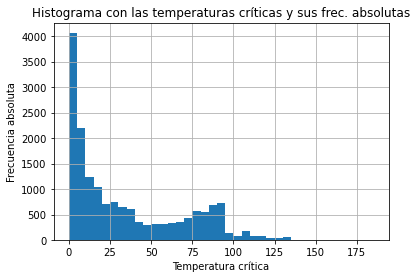
\includegraphics[width=\textwidth]{reg_hist_abs}
		\caption{Histograma con frecuencias absolutas}
	\end{subfigure}
	\begin{subfigure}{0.5\textwidth}
		\centering
		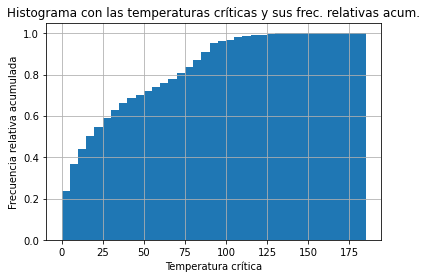
\includegraphics[width=\textwidth]{reg_hist_rel}
		\caption{Histograma con frecuencias relativas acumuladas}
	\end{subfigure}
	\caption{Histogramas con las temperaturas críticas de los superconductores}
	\label{fig:reg_histogramas}
\end{figure}

Los histogramas nos permiten ver que la gran mayoría de los datos de entrenamiento tienen temperaturas críticas inferiores a 20K (el 50\% de los datos aproximadamente). Por otro lado, los datos con temperaturas superiores a 95K se encuentran muy infrarepresentados, ya que constituyen menos del 5\% de los datos del conjunto de entrenamiento. Esto puede llegar a tener un impacto considerable en el ajuste del modelo, pues es posible que la hipótesis final que acabemos obteniendo no sea capaz de predecir correctamente aquellos datos cuya temperatura crítica se encuentre en los rangos con menos representación.


Ahora, aplicamos PCA y t-SNE para reducir la dimensionalidad y así poder representar la información más relevante contenida en los datos sobre un espacio bidimensional. Es condición necesaria que nuestro problema no tenga variables de tipo categórico, lo cual podemos ver que se cumple. Aplicaré los algoritmos sobre aquellos datos cuya temperatura crítica sea inferior a 95K, los cuales constituyen el 95.23\% de la muestra. Esto lo hago con el objetivo de no invertir una gran parte del rango de la barra de color de las gráficas en datos que apenas están representados.

Primero, he aplicado el algoritmo PCA (\textit{Principal Component Analysis}) para seleccionar aquellas dos componentes con máxima varianza. A continuación, sobre los resultados devueltos por PCA, he aplicado t-SNE (\textit{t-distributed Stochastic Neighbor Embedding}) para intentar agrupar datos con similitudes de forma que se vean cercanos al proyectarlos en el plano. En la figura \ref{fig:reg_pca_tsne} podemos ver las gráficas obtenidas.

\begin{figure}[h]
	\begin{subfigure}{0.5\textwidth}
		\centering
		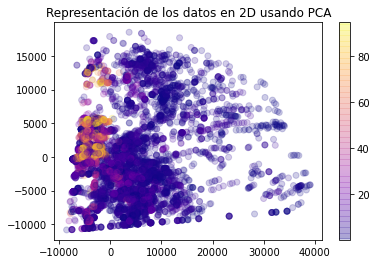
\includegraphics[width=\textwidth]{reg_pca}
		\caption{Representación obtenida por PCA}
	\end{subfigure}
	\begin{subfigure}{0.5\textwidth}
		\centering
		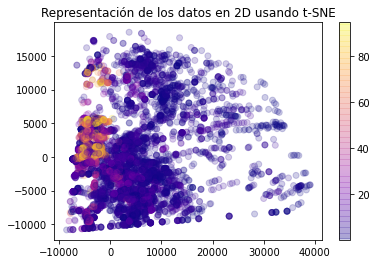
\includegraphics[width=\textwidth]{reg_tsne}
		\caption{Representación obtenida por t-SNE}
	\end{subfigure}
	\caption{Representación del conjunto de entrenamiento en 2 dimensiones mediante PCA y t-SNE}
	\label{fig:reg_pca_tsne}
\end{figure}

En la representación mediante PCA, podemos ver que a partir de las dos características con mayor variabilidad se consigue distinguir ligeramente de los datos con temperaturas más altas (que se encuentran más a la izquierda con colores rosados y anaranjados) del resto de datos. Por otro lado, vemos que la representación mediante t-SNE es prácticamente idéntica a la de PCA, luego deducimos que no se pueden agrupar datos similares únicamente a partir de las dos características más relevantes. Esto era algo esperable, pues al tener que predecir una variable continua, los datos se encuentran mucho menos separados unos de otros.





\subsection{Preprocesado de los datos}

En primer lugar, elimino las características cuya varianza sea menor que un umbral mediante \codeword{VarianceThreshold}. He decidido fijar este umbral a $10^{-3}$. Las características que no superen este umbral serán muy poco o nada relevantes en el proceso de aprendizaje, luego podemos eliminarlas sin problema.

A continuación, realizo una transformación de características no lineales. Concretamente, genero características polinomiales de grado 2 mediante \codeword{PolynomialFeatures}. No he considerado un grado más alto porque esto podría aumentar en exceso el número de características, lo cual podría provocar que nuestro modelo fuese demasiado complejo y que el tiempo que necesite para entrenar sea demasiado alto.

Después, realizo una estandarización de las características mediante \codeword{StandardScaler}. Esta estandarización consiste centrar y escalar cada característica restando su media y dividiendo por su desviación típica. El objetivo de esto es garantizar que las diferentes escalas de los datos originales no influyan negativamente en el ajuste del modelo y aumentar su velocidad de convergencia.

Por último, aplico de nuevo el algoritmo PCA para reducir el número de características. Seleccionamos el menor número de características que son capaces de explicar el 99.999\% de la variabilidad del conjunto de entrenamiento.

En la tabla \ref{fig:reg_preprocesado} se muestra cómo cambia el número de características a lo largo del preprocesado. Podemos ver que en el primer paso no se elimina ninguna característica porque su varianza sea demasiado baja. En cuanto a PCA se aprecia que, aunque el porcentaje de variabilidad a explicar que se ha fijado sea muy alto, el algoritmo elimina 2233 características, casi un 66\% de las características que estaban presentes en el paso anterior.

\begin{table}[h]
	\centering
	\begin{tabular}{|l|c|}
		\hline
		\multicolumn{1}{|c|}{\textbf{\begin{tabular}[c]{@{}c@{}}Pasos del\\ preprocesado\end{tabular}}} & \textbf{\begin{tabular}[c]{@{}c@{}}Número de \\ características\end{tabular}} \\ \hline
		Conjunto inicial                                                                                & 81                                                                            \\ \hline
		VarianceThreshold                                                                               & 81                                                                            \\ \hline
		PolynomialFeatures                                                                              & 3403                                                                          \\ \hline
		StandardScaler                                                                                  & 3403                                                                          \\ \hline
		PCA                                                                                             & 1170                                                                          \\ \hline
	\end{tabular}
	\caption{Evolución del número de características a lo largo del preprocesado}
	\label{fig:reg_preprocesado}
\end{table}

No he aplicado ningún mecanismo de eliminación de \textit{outliers} porque considero que los datos más alejados de la media aportan riqueza al conjunto de entrenamiento. Esta riqueza ayudará a que, durante el ajuste, se tengan en cuenta estos valores más atípicos y, por tanto, la hipótesis final será capaz de hallar una mejor predicción para ellos cuando aparezcan en el conjunto de test.

Para comprobar que hemos eliminado la dependencia lineal que pudiese haber entre las características, representamos las matrices de coeficientes de correlación de Pearson antes y después del preprocesado. Estas matrices se pueden ver en la figura \ref{fig:reg_pearson}.

\begin{figure}[h]
	\begin{subfigure}{0.5\textwidth}
		\centering
		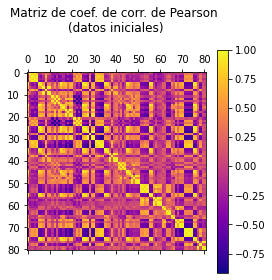
\includegraphics[width=\textwidth]{reg_pearson_antes}
		\caption{Antes del preprocesado}
	\end{subfigure}
	\begin{subfigure}{0.5\textwidth}
		\centering
		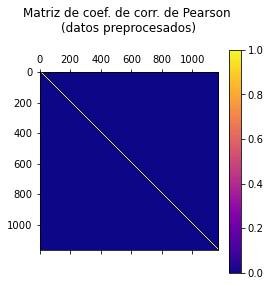
\includegraphics[width=\textwidth]{reg_pearson_despues}
		\caption{Después del preprocesado}
	\end{subfigure}
	\caption{Matrices de coeficientes de correlación de Pearson antes y después del preprocesado}
	\label{fig:reg_pearson}
\end{figure}

Se puede apreciar que, en la matriz resultante de aplicar el preprocesado, todos los coeficientes que no se encuentran en la diagonal principal tienen valores cercanos a 0, luego hemos eliminado conseguido eliminar la dependencia lineal entre características.

Este preprocesado será aplicado sobre ambos conjuntos de entrenamiento y de test. Para ello, primero es necesario ajustar los parámetros de las distintas funciones usadas en el preprocesado usando solamente el conjunto de entrenamiento.



\subsection{Modelo lineal}

El modelo lineal que usaré será Regresión Lineal, ya que es el único modelo lineal estudiado durante la asignatura que nos permite resolver un problema de regresión. Para este modelo, disponemos de dos algoritmos: SGD y Pseudoinversa. Me decanto por Pseudoinversa ya que el número de características que tendremos tras el preprocesado no es excesivamente grande, luego el orden de la matriz inversa que tendremos que calcular tampoco será demasiado alto.

La función de pérdida de este modelo es el error cuadrático medio (MSE) y tiene la siguiente expresión:

$$E(\textbf{w}) = \|\textbf{X}\textbf{w}-\textbf{y}\|^2$$

La ventaja de Pseudoinversa frente a SGD es que no necesitamos estimar hiperparámetros como la tasa de aprendizaje, el tamaño de minibatch o el número de épocas. Además, Pseudoinversa calcula aquellos pesos $w_{lin}$ que anulan el gradiente de la función de pérdida (el error cuadrático medio, MSE) dentro de la muestra.

$$\textbf{w}_{lin} = \textbf{X}^{\dag} \textbf{y} = (\textbf{X}^T \textbf{X})^{-1}\textbf{X}^T \textbf{y}$$ 

La clase de funciones que usamos son los polinomios de grado menor o igual que 2 aplicando un transformación de características no lineales en el preprocesado, como ya hemos visto. Esto nos permite obtener un modelo con una complejidad superior sin elevar en exceso el número de características.

\subsubsection{Regularización}

Es posible que aparezca sobreajuste debido al aumento de características con polinomios de grado 2, lo cual provoca que el modelo sea más complejo. Para intentar reducirlo, aplico la técnica de regularización \textit{weight decay}, que reduce la clase de funciones introduciendo una penalización sobre aquellas hipótesis cuyos pesos sean muy altos. Esta penalización se introduce en el modelo a través de un cambio en la fórmula para el cálculo de los pesos, que pasa a ser la siguiente ($\textbf{I}$ es la matriz identidad de orden el número de características más 1):

$$\textbf{w}_{lin} = (\textbf{X}^T \textbf{X} + \lambda \textbf{I})^{-1}\textbf{X}^T \textbf{y}$$

En esta fórmula aparece el parámetro de regularización $\lambda > 0$, que indica la intensidad con la que se aplica la regularización (cuanto mayor sea, mayor será la penalización aplicada sobre los pesos). Este será el único parámetro que tendremos que estimar más adelante para este modelo.

\subsection{Modelo no lineal usado para comparar}

Con el objetivo de comparar los resultados que obtendremos del modelo anteriormente descrito, también intentaré resolver el problema mediante otro modelo de regresión no lineal. Usaré un modelo de K-Nearest Neighbors adaptado a un problema de regresión. Este modelo predice la etiqueta para un dato calculando una interpolación de las etiquetas de aquellos datos del conjunto de entrenamiento que se encuentran más cercanos.

El modelo \codeword{KNeighborsRegressor} que proporciona \codeword{scikit-learn} permite fijar los pesos de la función de interpolación a \textit{uniform} (todos los puntos del vecindario tiene los mismos pesos) o a \textit{distance} (los puntos más cercanos tienen pesos mayores). Como este modelo depende enormemente de los datos del conjunto de entrenamiento, para intentar reducir el sobreajuste, considero que lo más apropiado es fijar los pesos a \textit{uniform}.

Por tanto, el único parámetro que tendremos que fijar para este modelo será el número de vecinos que se usarán en la interpolación.



\subsection{Métricas de error a usar}

Como hemos visto en los histogramas, la variable a predecir, temperatura crítica, toma valores en una escala muy amplia (desde 0 a 185). Esto puede provocar que el MSE no sea la métrica más adecuada para elegir la mejor hipótesis ya que puede verse muy afectada por esta escala al elevar las diferencias al cuadrado.

Por ello, he decidido que la métrica que usaré para seleccionar la mejor hipótesis hará uso del coeficiente de determinación $R^2$. Esta métrica es independiente de la escala de la variable a predecir, además de que tiene una fácil interpretación: La proporción de variabilidad que nuestro modelo es capaz de explicar frente a un modelo que siempre predice el valor medio. Su expresión es

$$R^2(modelo) = 1 - \frac{MSE(modelo)}{MSE(base)}$$

donde $modelo$ representa a nuestro modelo ajustado y $base$ representa al modelo que siempre predice el valor medio.

Al contrario que en MSE, lo que se persigue al usar la métrica $R^2$ es maximizarlo, es decir, que se acerque a 1 tanto como sea posible. Por tanto, usaré como métrica de error $E(modelo) = 1-R^2(modelo)$, pues minimizar esta expresión es equivalente a maximizar $R^2$. Podemos interpretar este valor como la proporción de variabilidad no explicada por nuestro modelo.

Además de $R^2$, también haré uso de la métrica MAE por su robustez, pues no es tan sensible como MSE a errores enormes provocados por valores atípicos. Esta métrica nos arroja información sobre la media de las distancias de los valores reales a los valores predichos por nuestra hipótesis final.





\subsection{Estimación de hiperparámetros y selección de la mejor hipótesis}

Utilizaremos Validación Cruzada para estimar los hiperparámetros de los modelos que queremos ajustar. Para ello, particiono el conjunto de entrenamiento en 5 \textit{folds} con el mismo tamaño y ajusto el modelo usando como conjunto de entrenamiento la unión de 4 \textit{folds}, dejando el restante como conjunto de validación. Para cada uno de los 5 modelos en los que dejo un \textit{fold} distinto para validación, calculo el error sobre el conjunto de entrenamiento y sobre el conjunto de validación, y luego hallo sus respectivos valores medios. Repetiré este procedimiento para cada combinación distinta de hiperparámetros que queramos probar, y me quedaré con aquella combinación de hiperparámetros que obtenga un menor error medio de validación.

La función de \codeword{scikit-learn} que he usado para implementar Validación Cruzada es \codeword{GridSearchCV}.

El modelo de regresión lineal solamente necesita estimar su parametro de regularización. En primer lugar, aplico Validación Cruzada para los valores 0.1, 1, 5, 10 y 20. En la figura \ref{fig:reg_plr_cv1} se muestran los resultados obtenidos.

\begin{table}[h]
	\centering
	\begin{tabular}{|c|c|c|}
		\hline
		\textbf{Valores de $\lambda$} & \textbf{$E_{in}$ medio} & \textbf{$E_{cv}$ medio} \\ \hline
		0.1                           & 0.1405                  & 0.17382                 \\ \hline
		1                             & 0.14104                 & 0.16448                 \\ \hline
		5                             & 0.14456                 & 0.15914                 \\ \hline
		10                            & 0.1479                  & 0.16016                 \\ \hline
		20                            & 0.15229                 & 0.16292                 \\ \hline
	\end{tabular}
	\caption{Errores de entrenamiento y de validación obtenidos en CV para Regresión Lineal (1)}
	\label{fig:reg_plr_cv1}
\end{table}

Podemos comprobar que se obtiene el menor $E_{cv}$ para $\lambda = 5$. Con el objetivo de afinar todavía más el valor de este parámetro, aplico de nuevo Validación Cruzada para los valores 4, 4.5, 5, 5.5 y 6. En la figura \ref{fig:reg_plr_cv2} se muestran los resultados obtenidos.

\begin{table}[h]
	\centering
	\begin{tabular}{|c|c|c|}
		\hline
		\textbf{Valores de $\lambda$} & \textbf{$E_{in}$ medio} & \textbf{$E_{cv}$ medio} \\ \hline
		4                             & 0.14374                 & 0.15927                 \\ \hline
		4.5                           & 0.14416                 & 0.15917                 \\ \hline
		5                             & 0.14456                 & 0.15914                 \\ \hline
		5.5                           & 0.14495                 & 0.15916                 \\ \hline
		6                             & 0.14533                 & 0.15921                 \\ \hline
	\end{tabular}
\caption{Errores de entrenamiento y de validación obtenidos en CV para Regresión Lineal (2)}
	\label{fig:reg_plr_cv2}
\end{table}

De nuevo, obtenemos que $\lambda = 5$ es el valor que arroja el menor $E_{cv}$, luego la mejor hipótesis para Regresión Lineal es aquella que obtenemos con este hiperparámetro. Sus errores medios en entrenamiento y validación son:

$E_{in} = 0.14456$

$E_{cv} = 0.15914$

Parece que hemos conseguido un buen ajuste, pues obtiene un $R^2$ medio sobre los conjuntos de validación igual a $1-0.15914=0.84086$. Por tanto, consigue explicar en media el 84.086\% de la variabilidad sobre dichos conjuntos.

Ahora, estimamos el único parámetro del modelo K-Neighbors Regressor, el número de vecinos $n$. Aplico Validación Cruzada para los valores 5, 10, 15 y 20. En la figura \ref{fig:reg_knr_cv} se muestran los resultados obtenidos.

\begin{table}[h]
	\centering
	\begin{tabular}{|c|c|c|}
		\hline
		\textbf{Valores de $n$} & \textbf{$E_{in}$ medio} & \textbf{$E_{cv}$ medio} \\ \hline
		5                       & 0.06811                 & 0.10748                 \\ \hline
		10                      & 0.09673                 & 0.12041                 \\ \hline
		15                      & 0.11246                 & 0.13075                 \\ \hline
		20                      & 0.1248                  & 0.13987                 \\ \hline
	\end{tabular}
	\caption{Errores de entrenamiento y de validación obtenidos en CV para K-Neighbors Regressor}
	\label{fig:reg_knr_cv}
\end{table}

Obtenemos que $n = 5$ es el valor que nos proporciona el menor $E_{cv}$. Sus errores medios en entrenamiento y validación son:

$E_{in} = 0.06811$

$E_{cv} = 0.10748$

Vemos que la hipótesis final de este modelo supera a la de Regresión Lineal, ya que su $R^2$ medio sobre los conjuntos de validación es igual a $1-0.10748=0.89252$. Por tanto, consigue explicar en media un 5\% más de la variabilidad que la otra hipótesis.

En una situación real, nos quedaríamos únicamente con el modelo K-Neighbors Regressor con $n=5$ por ser el mejor modelo según Validación Cruzada. Sin embargo, esta práctica está enfocada a modelos lineales, luego nos quedaremos también con el mejor modelo de Regresión Lineal.

Dado que en este apartado todavía no podemos usar el conjunto de test (pues lo reservamos para estimar el $E_{out}$ de la hipótesis final ajustada con todos los datos de entrenamiento), la estimación de $E_{out}$ que podemos dar por ahora es el $E_{cv}$ medio obtenido en Validación Cruzada.



\subsection{Obtención de la hipótesis final y estimación de $E_{out}$}

Finalmente, entrenamos la hipótesis final de Regresión Lineal con todo el conjunto de entrenamiento. Al evaluarla sobre el conjunto de entrenamiento, obtenemos las siguientes métricas:

$E_{in} = 0.14518$

$R^2_{in} = 0.85482$

$MAE_{in} = 8.81273$

A continuación, evaluamos la hipótesis final sobre el conjunto de test, obteniendo los siguientes resultados:

$E_{test} = 0.15344$

$R^2_{test} = 0.84656$

$MAE_{test} = 9.11804$

Como era esperable, el error en test aumenta ligeramente con respecto al de entrenamiento. Sin embargo, vemos que los porcentajes de variabilidad que nuestra hipótesis final es capaz de explicar en entrenamiento y en test difieren en menos de un 1\%. Además, vemos que la media de las distancias de los valores reales a los valores predichos se encuentra alrededor de los 9K, lo cual considero que es un dato bastante positivo teniendo en cuenta que el rango de temperaturas críticas llegaba hasta los 185K en el conjunto de entrenamiento.

Por último, vemos que la estimación de $E_{out}$ obtenida en este apartado ($E_{test}$) es ligeramente menor que la obtenida en el anterior ($E_{cv}$).

\subsubsection{Comparación con el modelo no lineal}

Después de ajustar la hipótesis final de KNR sobre todo el conjunto de entrenamiento, obtenemos las siguientes métricas al evaluarla sobre él:

$E_{in} = 0.06293$

$R^2_{in} = 0.93707$

$MAE_{in} = 4.69905$

Al evaluarla sobre el conjunto de test, obtenemos los siguientes resultados:

$E_{test} = 0.09081$

$R^2_{test} = 0.90919$

$MAE_{test} = 5.81234$

Podemos comprobar que en todas las métricas obtienen mejores resultados que la hipótesis final de Regresión Lineal. Concretamente, consigue explicar en test un 6\% más de variabilidad y su MAE en test es $3.3$K más bajo. A pesar de ello, considero que estas diferencias no son muy grandes y que, por tanto, el modelo lineal obtenido es relativamente bueno.

















\newpage

\section{Problema de Clasificación}

\subsection{Descripción del problema}

En este problema, se nos proporciona un conjunto de datos que contiene 49 características extraídas de 58509 señales eléctricas producidas por un motor. Este motor tiene algunos componentes intactos y otros defectuosos, los cuales se quiere clasificar 11 clases diferentes con condiciones distintas. Cada condición ha sido medida varias veces en 12 condiciones de funcionamiento diferentes (distintas velocidades, momentos de carga y fuerzas de carga). 

Para intentar comprender mejor las características que se manejan en este problema, he abierto el archivo en el que se encuentran. Al contrario que en el problema de regresión, en éste no encontramos una primera línea con los nombres de las características medidas. Lo único que podemos comprobar es que todas ellas son valores numéricos en coma flotante. La variable a predecir toma valores de 1 a 11, las 11 clases del problema. Esto pone de manifiesto que ésta es una variable discreta que toma un número finito de valores, luego es claramente un problema de clasificación.

Los elementos que constituyen este problema son los siguientes:

\begin{itemize}
	\item $X$: Conjunto de vectores con 49 valores numéricos en coma flotante que representan las características extraídas de las señales eléctricas producidas por un motor.
	\item $Y$: Conjunto de clases en que se quieren clasificar los distintos componentes del motor, $\{1,2,3,4,5,6,7,8,9,$ $10,11\}$.
	\item $f$: Función objetivo que asigna a cada vector de la población $X$ la clase a la que pertenece.
\end{itemize}






\subsection{Generación de conjuntos de entrenamiento, validación y test}

Partimos de un único archivo \codeword{Sensorless_drive_diagnosis.txt} (que he renombrado a \codeword{classification.txt}) con todos los datos, luego solo hay que generar los conjuntos de entrenamiento y test a partir del mismo. De nuevo, se puede comprobar que tampoco hay datos faltantes en este archivo por la misma razón que en problema anterior.

Al igual que antes, utilizo la función \codeword{train_test_split} para generar de forma aleatoria un conjunto de test con el 20\% y un conjunto de entrenamiento con el 80\% restante. Sin embargo, para evitar que haya clases infrarrepresentadas en cualquiera de los dos conjuntos, especifico que se mantenga la proporción de elementos en cada clase en ambos conjuntos mediante el parámetro \codeword{stratify}.

Hasta que no lleguemos al apartado de Validación Cruzada, no generaremos ningún conjunto de validación.





\subsection{Visualización del conjunto de entrenamiento}

Ya que tenemos poca información sobre el conjunto de datos, he decidido elaborar un histograma que estudia la variabilidad de cada una de las características. Concretamente, he clasificado las características según el orden de magnitud de sus varianzas. Los intervalos del histograma son de la forma $[10^{-k-1},10^{-k}]$ con $k \in \{0,\dots,8\}$. Podemos verlo en la figura \ref{fig:cla_hist}. Observamos que aproximadamente la mitad de las características tienen una varianza menor que $10^{-4}$. Esto será necesario tenerlo en cuenta en el preprocesado.

También considero importante saber la proporción de elementos de cada clase dentro del conjunto de entrenamiento. Para ello, confecciono un diagrama de barras con las frecuencias absolutas de cada clase. En la figura \ref{fig:cla_bar} podemos comprobar que las proporciones son las mismas para todas las clases.


\begin{figure}[h]
	\begin{subfigure}{0.5\textwidth}
		\centering
		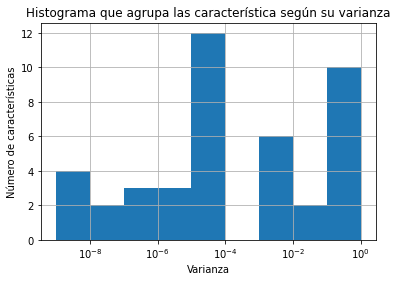
\includegraphics[width=\textwidth]{cla_hist}
		\caption{Histograma que agrupa las características según su varianza}
		\label{fig:cla_hist}
	\end{subfigure}
	\begin{subfigure}{0.5\textwidth}
		\centering
		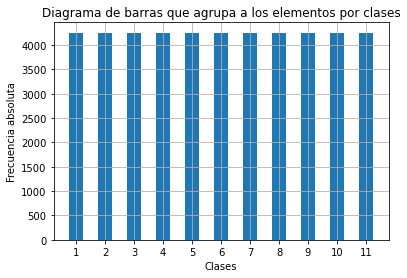
\includegraphics[width=\textwidth]{cla_bar}
		\caption{Diagrama de barras que agrupa a los elementos por clases}
		\label{fig:cla_bar}
	\end{subfigure}
\end{figure}

Por último, aplicamos PCA y t-SNE de forma análoga al problema anterior sobre la totalidad del conjunto de entrenamiento. Podemos ver los resultados obtenidos en la figura \ref{fig:cla_pca_tsne}.

\begin{figure}[h]
	\begin{subfigure}{0.5\textwidth}
		\centering
		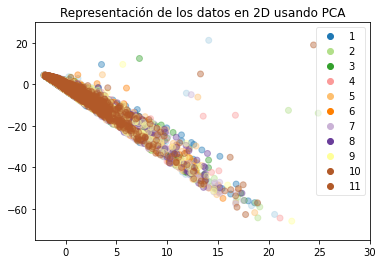
\includegraphics[width=\textwidth]{cla_pca}
		\caption{Representación obtenida por PCA}
	\end{subfigure}
	\begin{subfigure}{0.5\textwidth}
		\centering
		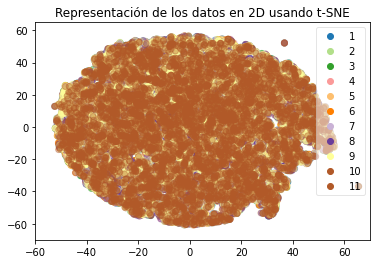
\includegraphics[width=\textwidth]{cla_tsne}
		\caption{Representación obtenida por t-SNE}
	\end{subfigure}
	\caption{Representación del conjunto de entrenamiento en 2 dimensiones mediante PCA y t-SNE}
	\label{fig:cla_pca_tsne}
\end{figure}

En la representación mediante PCA podemos ver que, exceptuando a unos pocos, la gran mayoría de los puntos con clases distintas se encuentran muy mezclados, siendo prácticamente imposible establecer zonas en las que solamente haya puntos de una única clase. Vemos que t-SNE intenta hacer una separación por clases, pero como era esperable, no tiene mucho éxito. Por tanto, podemos concluir que las dos características con mayor variabilidad sobre los datos no son suficientes como para separar los datos por clases de forma clara.






\subsection{Preprocesado de los datos}

Para este problema, aplicamos el preprocesado realizado en el problema de regresión por las mismas razones anteriormente expuestas: Eliminamos las características cuya varianza sea menor que un umbral, añadimos características polinomiales de grado 2, estandarizamos restando la media y dividiendo por la desviación típica de cada característica y aplicamos PCA para seleccionar el menor número de características que son capaces de explicar un determinado porcentaje de la variabilidad.

Como ya se vio en la figura \ref{fig:cla_hist}, necesitamos ser cuidadosos si queremos eliminar características con poca varianza. Según la información arrojada por el histograma, considero que un valor adecuado para el umbral es $10^{-7}$, pues solo elimina el 12.5\% de las características.

Por otro lado, el porcentaje de variabilidad de PCA lo he fijado a 99.9\%, lo cual reduce el número de características finales de 946 a 135, como se puede ver en la tabla \ref{fig:cla_preprocesado}. Considero que un porcentaje mayor provocaría que el número de características fuese demasido elevado.

\begin{table}[h]
	\centering
	\begin{tabular}{|l|c|}
		\hline
		\multicolumn{1}{|c|}{\textbf{\begin{tabular}[c]{@{}c@{}}Pasos del\\ preprocesado\end{tabular}}} & \textbf{\begin{tabular}[c]{@{}c@{}}Número de \\ características\end{tabular}} \\ \hline
		Conjunto inicial                                                                                & 48                                                                            \\ \hline
		VarianceThreshold                                                                               & 42                                                                            \\ \hline
		PolynomialFeatures                                                                              & 946                                                                          \\ \hline
		StandardScaler                                                                                  & 946                                                                          \\ \hline
		PCA                                                                                             & 135                                                                          \\ \hline
	\end{tabular}
	\caption{Evolución del número de características a lo largo del preprocesado}
	\label{fig:cla_preprocesado}
\end{table}

De nuevo, no he aplicado ningún mecanismo de eliminación de \textit{outliers} por la misma razón que en el problema anterior.

En la figura \ref{fig:cla_pearson} se representan las matrices de coeficientes de correlación de Pearson antes y después del preprocesado. Podemos comprobar que se ha eliminado la dependencia lineal entre características.

\begin{figure}[h]
	\begin{subfigure}{0.5\textwidth}
		\centering
		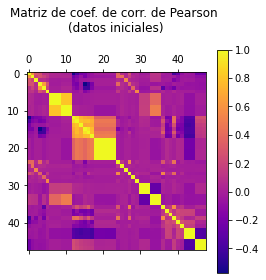
\includegraphics[width=\textwidth]{cla_pearson_antes}
		\caption{Antes del preprocesado}
	\end{subfigure}
	\begin{subfigure}{0.5\textwidth}
		\centering
		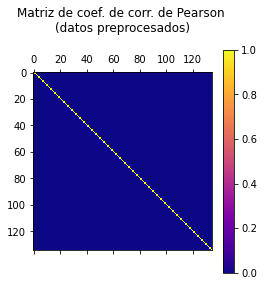
\includegraphics[width=\textwidth]{cla_pearson_despues}
		\caption{Después del preprocesado}
	\end{subfigure}
	\caption{Matrices de coeficientes de correlación de Pearson antes y después del preprocesado}
	\label{fig:cla_pearson}
\end{figure}






\subsection{Modelo lineal}

Dado que en el problema tenemos más de dos clases y que no sabemos si es separable, considero que el mejor modelo lineal para ajustar nuestra hipótesis es Regresión Logística Multinomial. Este modelo ajusta para cada clase $k \in \{1,\dots,11\}$ el hiperplano $\textbf{w}_k$ que mejor separa dicha clase del resto. La bondad de un conjunto de hiperplanos $\textbf{w}$ (matriz de hiperplanos $\textbf{w}_k$ puestos por filas) que separa cada clase del resto se mide a través del error de entropía cruzada multinomial, función de pérdida de este modelo:

$$E_{in}(\textbf{w}) = E_{in}(\textbf{w}_1,\dots,\textbf{w}_{11}) = - \frac{1}{N} \sum_{n=1}^{N} \sum_{k=1}^{11} y_{nk} \ln(\sigma(\textbf{w}_k^T \textbf{x}_n)) \qquad \text{donde } \sigma(t)=\frac{e^t}{1+e^t}$$

En la expresión anterior, las etiquetas $y_n$ del vector $\textbf{y}$ es necesario codificarlas como vectores one-hot, en los que $y_{nk} = 1$ si $y_n$ es la etiqueta asociada a la clase $k$ e $y_{nj} = 0$ para cualquier otro $j \neq k$.

Una vez calculados los hiperplanos, el modelo hace uso de la regla de clasificación \textit{Softmax}, que obtiene un vector con las probabilidades que un elemento tiene de pertenecer a cada una de las clases. A continuación, este elemento será clasificado en la clase cuya probabilidad sea mayor.

$$Softmax(\textbf{x}_n) = \left(\frac{\exp(\textbf{w}_1 \textbf{x}_n)}{\sum_{k=1}^{11}\exp(\textbf{w}_k \textbf{x}_n)},\dots,\frac{\exp(\textbf{w}_{11} \textbf{x}_n)}{\sum_{k=1}^{11}\exp(\textbf{w}_k \textbf{x}_n)}\right)$$

Para implementar el modelo, usaré el modelo \codeword{LogisticRegression} de \codeword{scikit-learn}. Este modelo cuenta con varios algoritmos que podemos elegir para ajustar nuestra hipótesis, de los cuales he decidido probar los dos siguientes:

\begin{itemize}
	\item \codeword{lbfgs}: Algoritmo de optimización quasi-Newton, de funciones con un gran número de parámetros o de gran complejidad. Solamente necesita la función a optimizar y su gradiente, pero no la matriz Hessiana. En cada iteración, el algoritmo busca una aproximación de la inversa de la matriz Hessiana.
	\item \codeword{saga}: Algoritmo de optimización que trabaja de forma muy similar a SGD actualizando los pesos mediante el gradiente de la función de pérdida.
\end{itemize}

También cuenta con otros parámetros como la tolerancia (error que es necesario alcanzar para que se dé el criterio de parada) o el número máximo de iteraciones, los cuales fijaré a 0.05 y 1000, respectivamente.

Al igual que antes, la clase de funciones a usar será los polinomios de grado menor o igual que 2.

\subsubsection{Regularización}

Para este modelo, intentaremos aplicar dos tipos de regularización diferentes: \textit{weight decay} o \textit{ridge} (que trabaja con la norma L2) y \textit{lasso} (que trabaja con la norma L1). La regularización se introduce en el modelo a través de una modificación en la función de pérdida (error aumentado).

\begin{itemize}
	\item \textit{Ridge} (L2): $E_{aug}(\textbf{w}) = E_{in}(\textbf{w}) + \lambda \|\textbf{w}\|_2^2$
	\item \textit{Lasso} (L1): $E_{aug}(\textbf{w}) = E_{in}(\textbf{w}) + \lambda \|\textbf{w}\|_1$
\end{itemize}

Por tanto, aparecen dos hiperparámetros que posteriormente será necesario ajustar: $\lambda>0$, que indica la intensidad de la regularización, y el tipo de penalización usada en la regularización (norma L1 o L2).


\subsection{Modelo no lineal usado para comparar}

Para este problema me he decantado por un clasificador de tipo SVM (Support Vector Machine) como modelo no lineal con el que comparar. A grandes rasgos, el objetivo de este modelo en el caso binario es encontrar un pasillo que mantenga un equilibrio entre su anchura y el número de puntos que se encuentran dentro de él. Podemos expresar su función de pérdida de la siguiente forma:

$$E(\textbf{w}) = \lambda \textbf{w}^T \textbf{w} + \frac{1}{N} \sum_{n=1}^{N} \max(1-y_n(\textbf{w}^T\textbf{x}_n+b),0)$$

El vector de pesos $(\textbf{w},b)$ representa el hiperplano sobre el que se centra el pasillo y $\lambda$ es su parámetro de regularización.

Como nuestro problema tiene más de dos clases, especifico que éste se resuelva mediante la estrategia \textit{One-vs-Rest}, que parte el problema en tantos problemas de clasificación binaria como clases haya. Para cada uno de ellos se entrena un modelo cuyo objetivo es determinar si un elemento pertenece o no pertenece a una clase concreta. Las predicciones se realizan usando el modelo que arroje una mayor confianza.

El kernel que usaré será RBF (\textit{Radial Base Function}). Para este kernel es necesario determinar un parámetro $\gamma>0$. Su expresión es la siguiente:

$$K(\textbf{x},\textbf{x}') = \exp(-\gamma\|\textbf{x}-\textbf{x}'\|^2)$$

Para implementarlo, usaré el modelo \codeword{SupportVectorClassification} que proporciona \codeword{scikit-learn}.





\subsection{Métricas de error a usar}

La métrica que usaré para seleccionar la mejor hipótesis será la Precisión o \textit{Accuracy} (porcentaje de elementos bien clasificados) por ser una medida directa y fácilmente interpretable. Además, al estar las clases perfectamente balanceadas, no tendremos situaciones en las que un modelo prediga correctamente las clases más representadas y cometa muchos errores con aquellas con menor representación. En este caso, la \textit{Accuracy} sería alta a pesar de que su porcentaje de fallos sea alto para las clases infrarrepresentadas.

Como la \textit{Accuracy} es una métrica a maximizar, tomaré el porcentaje de elementos mal clasificados como métrica para medir el error de una hipótesis: $E(modelo) = 1 - Accuracy(modelo)$.

También haré uso de la matriz de confusión $C$ para visualizar en qué tipo de predicciones nuestro modelo comete la mayor cantidad de errores. El valor $C_{i,j}$ situado en la fila $i$-ésima y la columna $j$-ésima se interpreta como la proporción de elementos cuya clase verdadera es $i$ pero que nuestro modelo predice como $j$. Por tanto, podemos ver la $Accuracy$ como la traza de la matriz de confusión. A partir de esta matriz, también calcularemos las siguientes dos métricas para cada clase $k$:

\begin{itemize}
	\item $Sensitivity_k$: Proporción de verdaderos positivos (elementos correctamente predichos en $k$) respecto al total de elementos pertenecientes a esa clase. Podemos calcularlo como $C_{k,k} / (\sum_{j=1}^{11} C_{j,k})$.
	\item $Specificity_k$: Proporción de verdaderos negativos (elementos correctamente predichos como no pertenecientes a $k$) respecto al total de elementos no pertenecientes a esa clase. Podemos calcularlo como ($\sum_{i \neq k} C_{i,i}) / (\sum_{i \neq k} \sum_{j=1}^{11} C_{j,i})$.
\end{itemize}



\subsection{Estimación de hiperparámetros y selección de la mejor hipótesis}

Empiezo aplicando Validación Cruzada sobre el modelo lineal. Es importante destacar que el algoritmo \codeword{saga} permite ambos tipos de regularización (L1 y L2), mientras que \codeword{lbfgs} solo permite L2. Por tanto, sobre este último no aplicaré regularización tipo L1. El hiperparámetro $\lambda$ tomará los valores 0.01, 0.1, 1 y 10. En la figura \ref{fig:cla_mlr_cv1} se muestran los resultados obtenidos.

\begin{table}[h]
	\centering
	\begin{tabular}{|c|c|c|c|c|}
		\hline
		\textbf{Algoritmo} & \textbf{Tipo de penalización} & \textbf{Valores de $\lambda$} & \textbf{$E_{in}$ medio} & \textbf{$E_{cv}$ medio} \\ \hline
		saga               & L1                            & 0.01                          & 0.55592                 & 0.55722                 \\ \hline
		saga               & L1                            & 0.1                           & 0.55649                 & 0.55742                 \\ \hline
		saga               & L1                            & 1                             & 0.55575                 & 0.55675                 \\ \hline
		saga               & L1                            & 10                            & 0.55593                 & 0.5568                  \\ \hline
		saga               & L2                            & 0.01                          & 0.55602                 & 0.55678                 \\ \hline
		saga               & L2                            & 0.1                           & 0.55527                 & 0.55643                 \\ \hline
		saga               & L2                            & 1                             & 0.55591                 & 0.55733                 \\ \hline
		saga               & L2                            & 10                            & 0.55561                 & 0.55656                 \\ \hline
		lbfgs              & L2                            & 0.01                          & 0.0242                  & 0.03512                 \\ \hline
		lbfgs              & L2                            & 0.1                           & 0.02494                 & 0.03431                 \\ \hline
		lbfgs              & L2                            & 1                             & 0.02979                 & 0.03705                 \\ \hline
		lbfgs              & L2                            & 10                            & 0.039                   & 0.04433                 \\ \hline
	\end{tabular}
	\caption{Errores de entrenamiento y de validación obtenidos en CV para Regresión Logística Multinomial (1)}
	\label{fig:cla_mlr_cv1}
\end{table}

Los mejores resultados son obtenidos con el algoritmo \codeword{lbfgs} usando regularización L2 con parámetro $\lambda = 0.1$. Podemos ver claramente que el algoritmo \codeword{lbfgs} consigue errores mucho más bajos que \codeword{saga} para todas las configuraciones del resto de parámetros. Por tanto, dejo fijo el algoritmo \codeword{lbfgs} con regularización L2 e intento afinar el valor de $\lambda$ aplicando otra vez Validación Cruzada. En la figura \ref{fig:cla_mlr_cv2} se muestran los resultados obtenidos.

\begin{table}[h]
	\centering
	\begin{tabular}{|c|c|c|c|c|}
		\hline
		\textbf{Algoritmo} & \textbf{Tipo de penalización} & \textbf{Valores de $\lambda$} & \textbf{$E_{in}$ medio} & \textbf{$E_{cv}$ medio} \\ \hline
		lbfgs              & L2                            & 0.05                          & 0.0246                  & 0.03448                 \\ \hline
		lbfgs              & L2                            & 0.1                           & 0.02494                 & 0.03431                 \\ \hline
		lbfgs              & L2                            & 0.3                           & 0.0266                  & 0.03523                 \\ \hline
		lbfgs              & L2                            & 0.5                           & 0.02778                 & 0.03608                 \\ \hline
		lbfgs              & L2                            & 0.7                           & 0.02871                 & 0.03662                 \\ \hline
	\end{tabular}
	\caption{Errores de entrenamiento y de validación obtenidos en CV para Regresión Logística Multinomial (2)}
	\label{fig:cla_mlr_cv2}
\end{table}


De nuevo, obtenemos que $\lambda = 0.1$ es el valor que arroja el menor $E_{cv}$, luego esta será la configuración de hiperparámetros que mantengamos para el modelo de Regresión Logística Multinomial. Sus errores medios en entrenamiento y validación son:

$E_{in} = 0.02494$

$E_{cv} = 0.03431$

Considero que esta primera hipótesis que hemos obtenido con Validación Cruzada es bastante buena, pues obtiene un 96.569\% de $Accuracy$ medio sobre los conjuntos de validación.

Ahora, estimamos los parámetros del modelo Support Vector Classification. Los valores que daré a $\lambda$ serán 0.01, 0.1, 1 y 10, mientras que $\gamma$ podrá tomar los valores 0.001 y \textit{scale} (este último toma $\gamma = 1/q$, donde $q=135$ es el número de características). En la figura \ref{fig:cla_svc_cv} se muestran los resultados obtenidos.

\begin{table}[h]
	\centering
	\begin{tabular}{|c|c|c|c|}
		\hline
		\textbf{Valores de $\gamma$} & \textbf{Valores de $\lambda$} & \textbf{$E_{in}$ medio} & \textbf{$E_{cv}$ medio} \\ \hline
		0.001                        & 0.01                          & 0.00278                 & 0.01651                 \\ \hline
		0.001                        & 0.1                           & 0.0092                  & 0.0194                  \\ \hline
		0.001                        & 1                             & 0.02911                 & 0.03807                 \\ \hline
		0.001                        & 10                            & 0.12346                 & 0.12765                 \\ \hline
		scale                        & 0.01                          & 0.00241                 & 0.01664                 \\ \hline
		scale                        & 0.1                           & 0.00863                 & 0.01927                 \\ \hline
		scale                        & 1                             & 0.02786                 & 0.03752                 \\ \hline
		scale                        & 10                            & 0.12098                 & 0.12496                 \\ \hline
	\end{tabular}
	\caption{Errores de entrenamiento y de validación obtenidos en CV para Support Vector Classification}
	\label{fig:cla_svc_cv}
\end{table}

Obtenemos que $\gamma = 0.001$ y $\lambda = 0.01$ nos proporcionan el menor $E_{cv}$. Sus errores medios en entrenamiento y validación son:

$E_{in} = 0.00278$

$E_{cv} = 0.01651$

Vemos que el Accuracy en validación de la hipótesis final de este modelo es 98.349\%, superando en casi un 2\% a la hipótesis de Regresión Logística Multinomial.

De nuevo, nos quedamos con las mejores hipótesis de cada modelo para compararlas sobre el conjunto de test. Consideramos que las estimaciones de $E_{out}$ en este apartado son los $E_{cv}$ medios correspondientes a cada hipótesis.





\subsection{Obtención de la hipótesis final y estimación de $E_{out}$}

Entrenamos la hipótesis final de Regresión Logística Multinomial con todo el conjunto de entrenamiento. Luego, la evaluamos sobre los conjuntos de entrenamiento y de test. Podemos ver a continuación las métricas de error, \textit{Accuracy}, matriz de confusión (figura \ref{fig:cla_confusion_mlr}), \textit{Sensitivity} y \textit{Specificity} (tabla \ref{fig:cla_sensit_specif_mlr}).

$E_{in} = 0.02628$

$Accuracy_{in} = 0.97372$

$E_{test} = 0.03162$

$Accuracy_{test} = 0.96838$

Empezamos viendo que la hipótesis final obtiene un error de 3.162\% en test, inferior al 3.431\% obtenido en Validación Cruzada. Por tanto, hemos obtenido una mejor estimación de $E_{out}$ (nuestra hipótesis final tiene casi un 0.3\% más de \textit{Accuracy} que la obtenida en Validación Cruzada). Por otro lado, vemos que los errores en entrenamiento y en test solo difieren en un 0.5\% aproximadamente, luego se puede inferir que la hipótesis final se ve muy poco perjudicada por el sobreajuste.

\begin{figure}[h]
	\begin{subfigure}{0.5\textwidth}
		\centering
		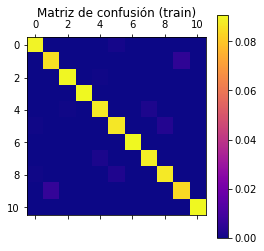
\includegraphics[width=\textwidth]{cla_confusion_mlr_train}
		\caption{Entrenamiento}
	\end{subfigure}
	\begin{subfigure}{0.5\textwidth}
		\centering
		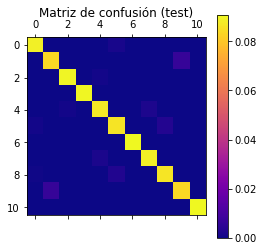
\includegraphics[width=\textwidth]{cla_confusion_mlr_test}
		\caption{Test}
	\end{subfigure}
	\caption{Matrices de confusión para Multinomial Logistic Regression}
	\label{fig:cla_confusion_mlr}
\end{figure}

Como era esperable después de ver la \textit{Accuracy}, las matrices de confusión son casi idénticas y tienen valores cercanos a 0 en todas aquellas posiciones que no forman parte de la diagonal principal. Si las observamos en mayor profundidad, vemos tonalidades ligeramente más claras de azul en las posiciones que involucran a las parejas de clases (2,10), (5,8) y (6,9). Esto significa que nuestro modelo encuentra una ligera dificultad para distinguir entre estas parejas de clases.

\begin{table}[h]
	\centering
	\begin{tabular}{|c|c|c|c|c|}
		\hline
		\textbf{Clase} & \textbf{Sensitivity$_{in}$} & \textbf{Specificity$_{in}$} & \textbf{Sensitivity$_{test}$} & \textbf{Specificity$_{test}$} \\ \hline
		\textbf{1}     & 0.98705                     & 0.97239                     & 0.98208                       & 0.96702                       \\ \hline
		\textbf{2}     & 0.92849                     & 0.97831                     & 0.92192                       & 0.97302                       \\ \hline
		\textbf{3}     & 0.9953                      & 0.97156                     & 0.98871                       & 0.96635                       \\ \hline
		\textbf{4}     & 0.99836                     & 0.97126                     & 0.99623                       & 0.9656                        \\ \hline
		\textbf{5}     & 0.97144                     & 0.97395                     & 0.96422                       & 0.9688                        \\ \hline
		\textbf{6}     & 0.95567                     & 0.97553                     & 0.94585                       & 0.97065                       \\ \hline
		\textbf{7}     & 1                           & 0.97109                     & 1                             & 0.96523                       \\ \hline
		\textbf{8}     & 0.9726                      & 0.97383                     & 0.97106                       & 0.96811                       \\ \hline
		\textbf{9}     & 0.96332                     & 0.97476                     & 0.95943                       & 0.96927                       \\ \hline
		\textbf{10}    & 0.9389                      & 0.97716                     & 0.923                         & 0.97292                       \\ \hline
		\textbf{11}    & 1                           & 0.97109                     & 1                             & 0.96522                       \\ \hline
	\end{tabular}
	\caption{Valores de \textit{Sensitivity} y \textit{Specificity} para Multinomial Logistic Regression}
	\label{fig:cla_sensit_specif_mlr}
\end{table}

En primer lugar, vemos que los valores de \textit{Sensitivity} tanto en entrenamiento como en test son ligeramente más bajos (entre 92\% y 98\%) en las clases 2, 10, 5, 8, 6 y 9 por lo previamente dicho al analizar las matrices de confusión. El resto de clases tienen porcentajes superiores al 98\%, incluso alcanzándose el 100\% en las clases 7 y 11. En cuanto a Specificity, no vemos grandes diferencias entre los porcentajes obtenidos por las diferentes clases, aunque sí observamos que de entrenamiento a test estos porcentajes disminuyen alrededor de un 0.5\%.

En general, parece que hemos obtenido un modelo lineal de una calidad bastante alta.



\subsubsection{Comparación con el modelo no lineal}

Ahora, ajustamos la hipótesis final de Support Vector Classification sobre todo el conjunto de entrenamiento, y la evaluamos sobre los conjuntos de entrenamiento y de test. Podemos ver a continuación las métricas de error, \textit{Accuracy}, matriz de confusión (figura \ref{fig:cla_confusion_svc}), \textit{Sensitivity} y \textit{Specificity} (tabla \ref{fig:cla_sensit_specif_svc}).

$E_{in} = 0.00259$

$Accuracy_{in} = 0.99741$

$E_{test} = 0.01307$

$Accuracy_{test} = 0.98693$

Empezamos viendo que la \textit{Accuracy} en test supera en casi un 2\% a la obtenida en el modelo lineal, (lo cual no nos extraña, pues es un modelo no lineal y su potencia debería ser mayor). En este caso, el 1.307\% de error en test también mejora al 1.651\% obtenido en Validación Cruzada. Parece que hay un poco más de sobreajuste que en modelo lineal, pues los errores de entrenamiento y de test difieren en aproximadamente un 1\%.

\begin{figure}[h]
	\begin{subfigure}{0.5\textwidth}
		\centering
		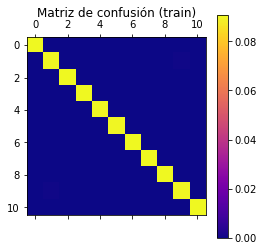
\includegraphics[width=\textwidth]{cla_confusion_svc_train}
		\caption{Entrenamiento}
	\end{subfigure}
	\begin{subfigure}{0.5\textwidth}
		\centering
		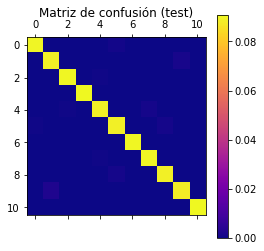
\includegraphics[width=\textwidth]{cla_confusion_svc_test}
		\caption{Test}
	\end{subfigure}
	\caption{Matrices de confusión para Support Vector Classification}
	\label{fig:cla_confusion_svc}
\end{figure}

Observamos que las matrices de confusión son muy parecidas a las obtenidas en el modelo lineal. Cabe destacar que las tonalidades más claras de azul que apreciábamos en el modelo lineal, aquí desaparecen en entrenamiento, y en test podemos verlas pero mucho más disimuladas.

\begin{table}[h]
	\centering
	\begin{tabular}{|c|c|c|c|c|}
		\hline
		\textbf{Clase} & \textbf{Sensitivity$_{in}$} & \textbf{Specificity$_{in}$} & \textbf{Sensitivity$_{test}$} & \textbf{Specificity$_{test}$} \\ \hline
		\textbf{1}     & 0.99812                     & 0.99734                     & 0.99153                       & 0.98647                       \\ \hline
		\textbf{2}     & 0.99297                     & 0.99786                     & 0.96846                       & 0.9888                        \\ \hline
		\textbf{3}     & 0.99929                     & 0.99723                     & 0.99343                       & 0.98627                       \\ \hline
		\textbf{4}     & 0.99953                     & 0.9972                      & 0.99812                       & 0.98581                       \\ \hline
		\textbf{5}     & 0.99718                     & 0.99744                     & 0.98673                       & 0.98694                       \\ \hline
		\textbf{6}     & 0.996                       & 0.99756                     & 0.97653                       & 0.98797                       \\ \hline
		\textbf{7}     & 1                           & 0.99716                     & 1                             & 0.98562                       \\ \hline
		\textbf{8}     & 0.99648                     & 0.99751                     & 0.98411                       & 0.98721                       \\ \hline
		\textbf{9}     & 0.99648                     & 0.99751                     & 0.98581                       & 0.98704                       \\ \hline
		\textbf{10}    & 0.99552                     & 0.9976                      & 0.98194                       & 0.98742                       \\ \hline
		\textbf{11}    & 1                           & 0.99716                     & 0.98977                       & 0.98664                       \\ \hline
	\end{tabular}
	\caption{Valores de \textit{Sensitivity} y \textit{Specificity} para Support Vector Classification}
	\label{fig:cla_sensit_specif_svc}
\end{table}

Por último, los valores de \textit{Sensitivity} son todos superiores al 99\% en entrenamiento, pero en test disminuyen ligeramente justo en aquellas clases con las que el modelo lineal encontraba una mayor dificultad. Los porcentajes de \textit{Specificity} son aproximadamente un 2\% mayores que los del modelo lineal y, al igual que antes, disminuyen ligeramente de entrenamiento a test.

En general, vemos que la hipótesis final de Support Vector Classification se comporta de forma muy parecida a la de Multinomial Logistic Regression, aunque obteniendo resultados algo superiores. Sin embargo, considero que la hipótesis final del modelo lineal arroja unos resultados muy satisfactorios, ya que las diferencias entre ambas hipótesis son muy leves, además de que las pequeñas carencias que encontrabamos en el modelo lineal también las vemos reflejadas en el no lineal.



\end{document}



